\documentclass{article}

\usepackage{amsmath}
\usepackage{graphicx}

\graphicspath{ {./images/} }

\author{Ashrit Yarava}
\title{Fuzzy Sets - Assignment 1}

\begin{document}

\maketitle
	
\begin{enumerate}
	\item Suggest a fuzzy set (membership function) of the concept of "high temperature in summer in edmonton. Use LLMs (atleast two versions) to elicit a fuzzy set describing this concept. Discuss the prompts used and interpret the result(s).
	
	Temperatures in edmonton during the summer range from a low of $10^{\circ}$ C to $22^{\circ} C$. The function below accounts for all high temperatures during the summer, even temperatures we might not have seen, since temperatures higher than the above range would also be considered summer. The memebrship functio for this range could be described as a $\Gamma$-membership function given below:
	
	\[
		A(x) = \left \{\begin{matrix}
			0 & \text{if } x \leq 10\\
			1 - e^{-10(x - 10)^2} & \text{if } x > 10
		\end{matrix} \right \}
	\]
	
	The first LLM, ChatGPT, was used to generate the following fuzzy set making use of a trapezoidal fuzzy set:
	
	\[
		\mu_\text{summer} (T) = \left \{\begin{matrix}
			0 & T \leq 15, \\
			\frac{T - 15}{5} & 15 < T < 20, \\
			1 & 20 \leq T \leq 27, \\
			\frac{33 - T}{6} & 27 \leq T \leq 23, \\
			0 & T \leq 23
		\end{matrix} \right \}
	\]
	
	The second LLM, Google Gemini, produces the following result:
	
	\[
		\mu(x) = \left \{\begin{matrix}
			0 & \text{if } x \leq 12 \\
			0.5 & \text{if } 12 < x \leq 18 \\
			1 & \text{if } 18 < x \leq 24 \\
			0.5 & \text{if } 24 < x \leq 30 \\
			0 & \text{if } x > 30 \\
		\end{matrix}\right\}
	\]
	
	The prompt used for both LLMs to generate the result was: "Write a fuzzy set membership function describing the summer temperature in Edmonton, Alberta." Both of the LLMs make the assumption that there is a maximimum temperature that should be considered summer. Personally, I don't believe this to be the case, as my function accounts for warmer temperatures being considered summer as well. The LLMs also state that the low temperature considered for summer is higher than weather statistics report.
	
	\item Given the fuzzy set defined in the space of real numbers $\mathcal{R}$ with the following membership function:
	
	\[
		A = \exp (-\frac{(x-1)^2}{4}) = \exp(-\frac1 4(x - 1)^2)
	\]
	
	Determine the following:
	\begin{itemize}
		\item Energy measure of fuzziness of $A$, $E(A)$; use $e(u) = u$
		
		\[
			\begin{matrix}
				E(A) =& \int_X e[A(x_i)] \, \text{d}x \\
				\\
				E(A) =& \int_{-\infty}^{\infty} \exp(-\frac{1}{4} (x - 1)^2) \, \text{d}x \\
				\\
				E(A) =& 2 \sqrt \pi
			\end{matrix}
		\]
		
		\item Entropy measure of fuzziness of $A$, $H(A)$; use $h(u) = 4u(1 - u)$

		\[
			\begin{matrix}
				H(A) =& \int_X h[A(x_i)] \, \text{d} x \\
				\\
				H(A) =& \int_X 4(A(x)(1-A(x)) \, \text{d} x \\
				\\
				H(A) =& 4 \int_X A(x)-A(x)^2 \, \text{d} x \\
				\\
				H(A) =& 4 \int_{-\infty}^{\infty} \exp(-\frac1 4(x - 1)^2)-\exp(-\frac1 4(x - 1)^2)^2 \, \text{d} x \\
				\\
				H(A) =& 4(2 + \sqrt2)\sqrt\pi \\
				\\
				H(A) =& 8\sqrt\pi + 4\sqrt{2\pi}
			\end{matrix}
		\]

		\item $\alpha$-cut of $A$ for $\alpha = 0.5$ and a strong $\alpha$-cut for $\alpha = 0.4$

		The $\alpha$-cut of $A$ at $\alpha = 0.5$ would be $[1 - 2\sqrt{\ln2}, 1 + 2\sqrt{\ln2}]$. The strong $\alpha$-cut at $\alpha = 0.4$ would be $(1 - 2\sqrt{\ln5 -\ln2}, 1 + 2\sqrt{\ln5 -\ln2})$.

		\item Core and support of $A$
		
		The support of $A$ would be $\mathcal{R}$. And the core of the fuzzy set would be $\{1\}$.
		
	\end{itemize}
	
	Is this fuzzy set normal?
	
	The fuzzy set is considered normal since $\text{hgt}(A)=1$.
	
	\item Multi-Part Question:
	
	\begin{enumerate}
		\item Determine the specificity of the fuzzy set of $A$ with the membership function defined over $[0, 20]$. Assume the range is 20.

		\[
			A(x) = \left\{ \begin{matrix}
				1 - \frac x 8 & \text{if } x \in [0, 8] \\
				0 & \text{otherwise} 
			\end{matrix} \right\}
		\]
		
		To calculate the specificity of $A$, first identify a suitable value for $\alpha$ in $\int_0^1 \text{sp}(A_\alpha) \, \text{d}\alpha$. In this case, choose $\alpha = 1 - \frac x 8$, such that $x= 8(1 -\alpha)$.
		
		\[
		\begin{matrix}
			\int_0^1 \text{sp}(A_\alpha) \, \text{d} \alpha \\
			\\
			\text{sp}(A_{1 - \frac x 8}) = 1 - \frac{2(1 - \alpha)}{5}\\
			\\
			\int_0^1 \frac 3 5 + \frac 2 5 \alpha \, \text{d} \alpha\\
			\\
			\text{sp}(A) = 0.8
		\end{matrix}
		\]
		
		\item Find the characteristic function of $B$ such that the specificity of $B$ is equal to the specificity of $A$.

		\[
			B(x) = \left\{ \begin{matrix}
				1 & \text{if } x \in [0, b] \\
				0 & \text{otherwise}
			\end{matrix} \right\}
		\]
		
		If $B$ has an unspecified range, then the characteristic function would be:
		
		\[
			B(x) = \left \{ \begin{matrix}
				1 & \text{if } x \in [0, 0.2(range)]\\
				0 & \text{otherwise}
			\end{matrix} \right \}
		\]
		
		However, if $B$ has the same range as $A$, then the bounds for $x$ in the above piecewise function would become $x \in [0, 4]$.

	\end{enumerate}
	
	\item Given the intervals $A = [-4, 0], B=[-4, 5], C=[-1, 6]$. Compute:
	
	\begin{enumerate}
	
		\item $A + B, 2A + CB$
		
		\[
		\begin{matrix}
			A + B\\
			[-4 + -4, 0 + 5]\\
			[-8, 5]
		\end{matrix}
		\]
		
		\[
		\begin{matrix}
			2A + CB\\
			2([-4, 0]) + ([-1, 6])([-4, 5])\\
			[-8, 0] + [\min(4, -5, -24, 30), \max(4, -5, -24, 30)]\\
			[-8, 0] + [-24, 30]\\
			[-32, 30]
		\end{matrix}
		\]
		
		\item $nA$, $n > 0$. Determine the specificity of $A + A + \dots + A$ (n-fold addition of $A$); how does the specificity of the result depend on the value of $n$. Assume that th evalue of \textit{range} is given.
	
		Take range, $r$ to be a constant.
		
		For $n = 1$: The specificity is $\text{sp}(A) = 1 - \frac{0 - (-4)}{r} = 1 - \frac 4 r$

		For $n = 2$: $A + A = [-8, 0]$. The specificity is $\text{sp}(A + A) = 1 - \frac{0 - (-8)}{r} = 1 - \frac 8 r$
		
		For $n = 3$: $A + A + A = [-12, 0]$. The specificity is $\text{sp}(A + A) = 1 - \frac{0 - (-12)}{r} = 1 - \frac 12 r$.
		
		From the above pattern, the specificity for $n$-fold addition of $A$ can be defined to be: $1 - \frac{4n}{r}$.
	
	\end{enumerate}
	
	\item Given are fuzzy sets $A$ and $B$ shown in the figures below:

	Plot the intersection $A \cap B$ by considering the following $t$-norms: minimum, product, Lukasiewicz, drastic product.
	
	\textit{Plots provided on the next page.}
	
	\begin{figure}[h]
		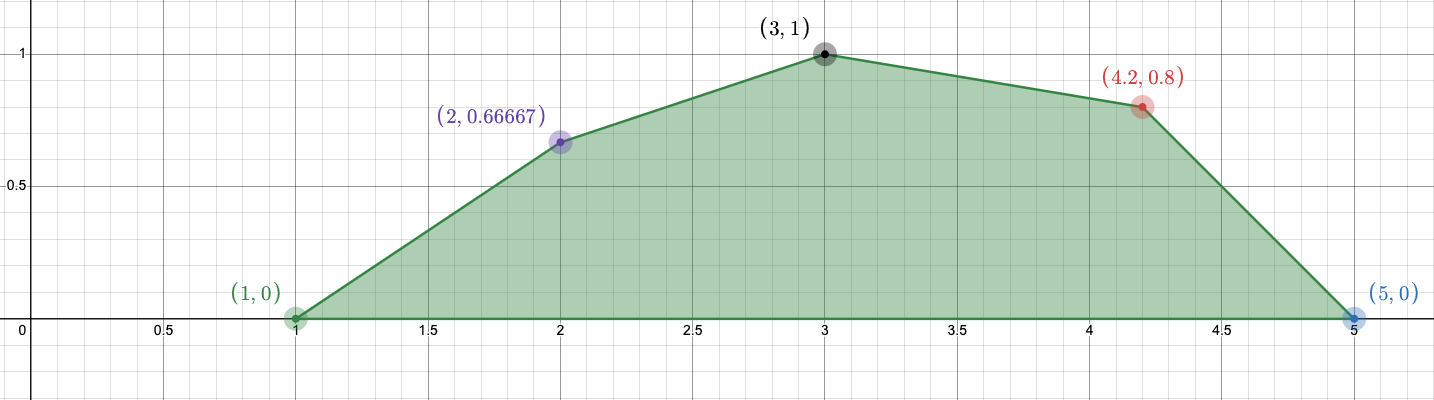
\includegraphics[width=\textwidth]{1.5_min.png}
		\caption{Minimum Plot.}
		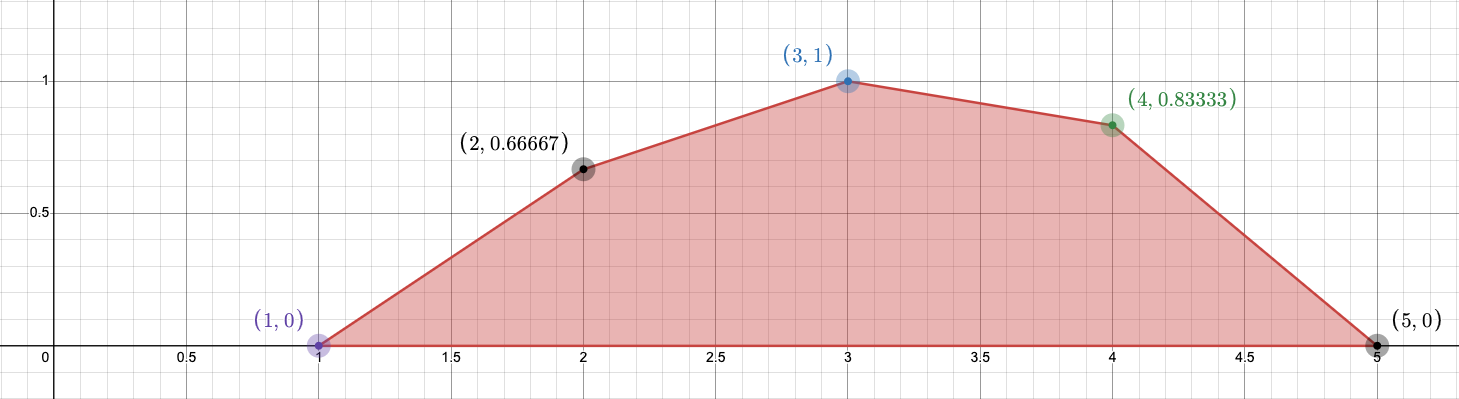
\includegraphics[width=\textwidth]{1.5_product.png}
		\caption{Product Plot.}
		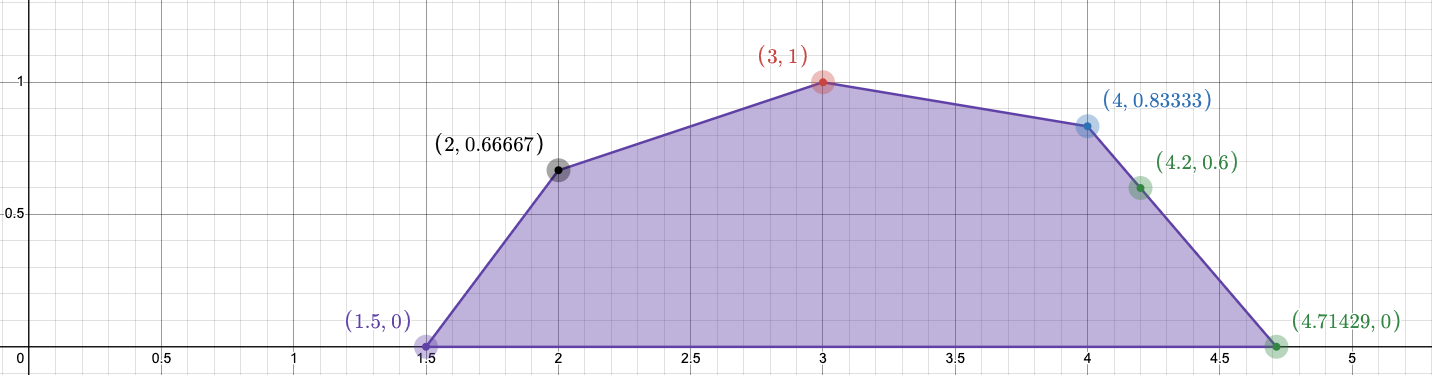
\includegraphics[width=\textwidth]{1.5_lukasiewicz.png}
		\caption{Lukasiewicz Plot.}
		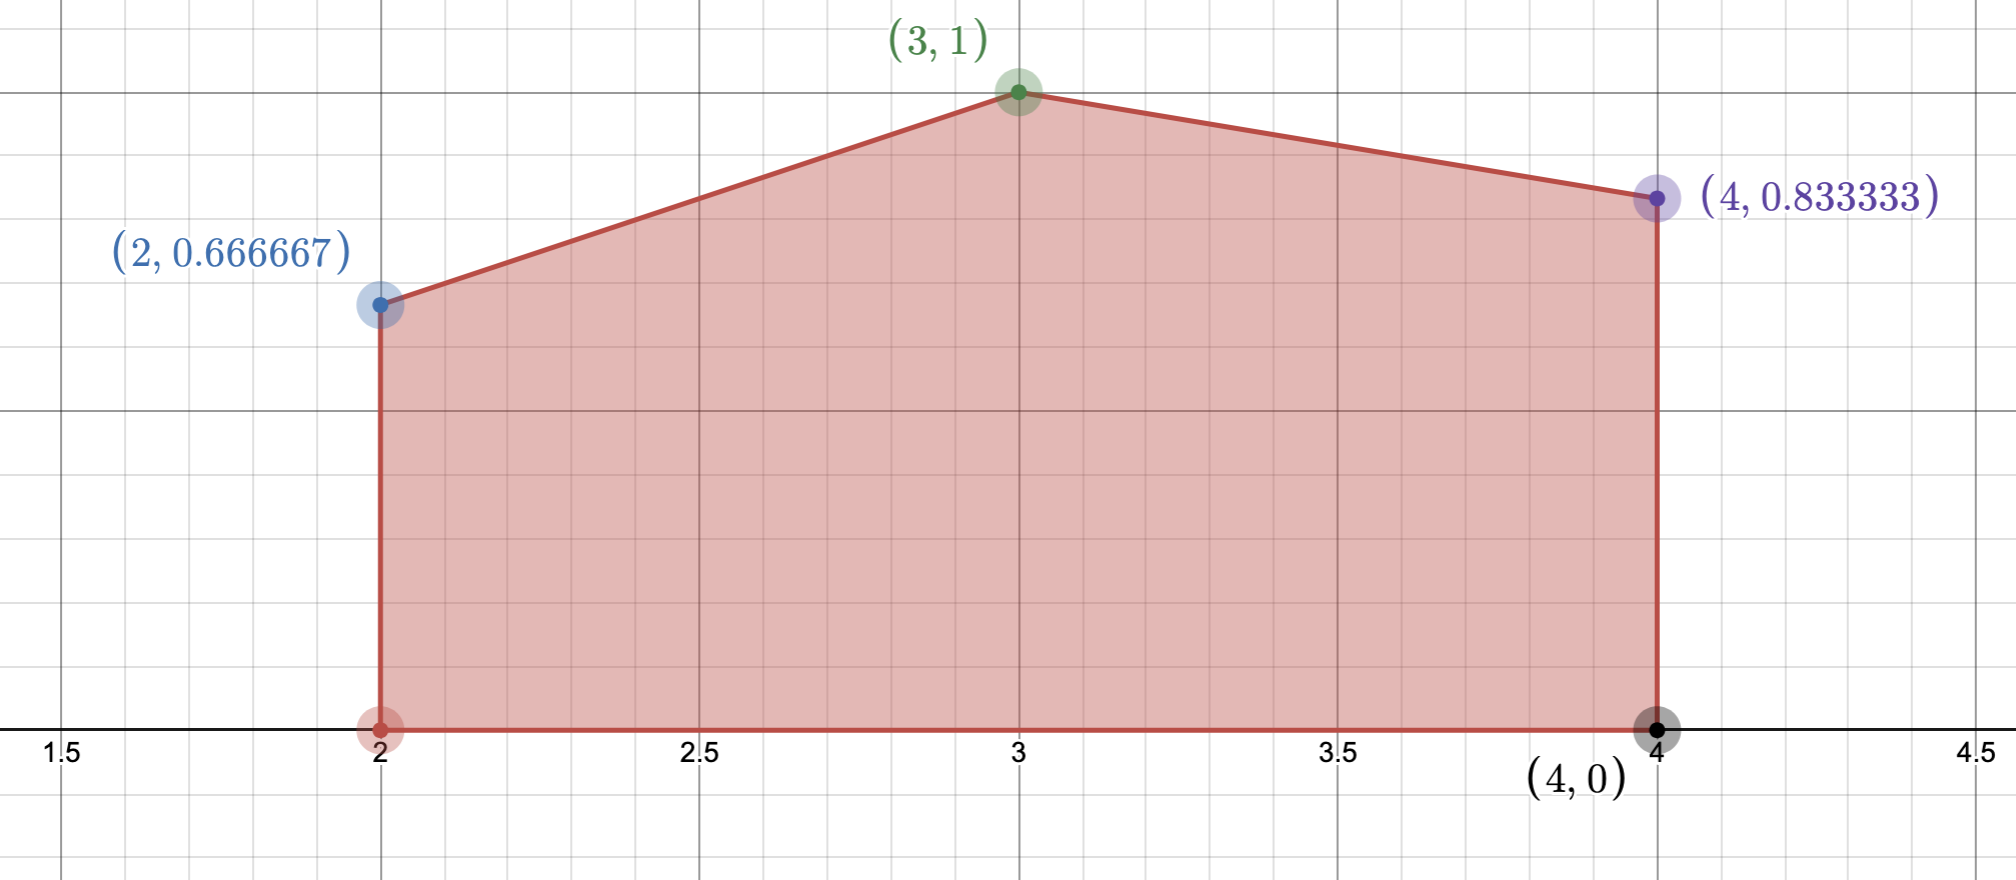
\includegraphics[width=\textwidth]{1.5_drastic.png}
		\caption{Drastic Plot.}
	\end{figure}
	
\end{enumerate}
	
\end{document}